\chapter{Methodology}

\section{Research Design Overview}

This research follows a mixed-methods approach combining corpus linguistics, formal methods, and empirical evaluation. The methodology is structured into four phases:

\begin{enumerate}
    \item \textbf{Phase 1: Corpus Construction and Pattern Discovery} -- Extract and annotate policy rules, identify formalizability patterns
    \item \textbf{Phase 2: Translation Pipeline Development} -- Design and implement the Policy $\rightarrow$ FOL $\rightarrow$ SHACL transformation
    \item \textbf{Phase 3: Verification Framework} -- Establish validation checkpoints and formal verification mechanisms
    \item \textbf{Phase 4: Evaluation} -- Measure coverage, accuracy, and effectiveness
\end{enumerate}

% Methodology Diagram
\begin{figure}[h]
\centering
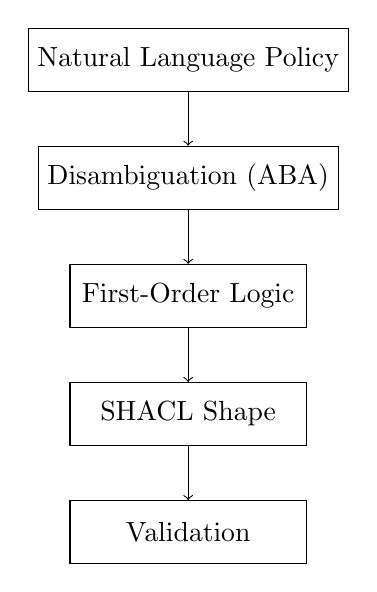
\begin{tikzpicture}[
    node distance=1.5cm,
    box/.style={rectangle, draw, minimum width=3cm, minimum height=0.8cm}
]
    \node[box] (policy) {Natural Language Policy};
    \node[box, below of=policy] (disamb) {Disambiguation (ABA)};
    \node[box, below of=disamb] (fol) {First-Order Logic};
    \node[box, below of=fol] (shacl) {SHACL Shape};
    \node[box, below of=shacl] (valid) {Validation};
    
    \draw[->] (policy) -- (disamb);
    \draw[->] (disamb) -- (fol);
    \draw[->] (fol) -- (shacl);
    \draw[->] (shacl) -- (valid);
\end{tikzpicture}
\caption{High-level transformation pipeline}
\end{figure}

\section{Phase 1: Corpus Construction and Pattern Discovery}

\subsection{Data Collection}

Policy rules are extracted from the following AIT documents:

\begin{table}[h]
\centering
\caption{Source Documents for Corpus}
\begin{tabular}{llc}
\toprule
Document Code & Title & Est. Rules \\
\midrule
FB-6-1-1 & Credit Policy & 35-40 \\
FS-1-1-1 & Campus Accommodation for Students & 60-65 \\
AA-4-1-1 & Academic Integrity in Research & 8-10 \\
PA-2-1-2 & Ethical Behavior and Grievance & 45-50 \\
-- & Student Handbook & 350+ \\
\bottomrule
\end{tabular}
\end{table}

\subsection{Annotation Scheme}

Each extracted rule is annotated along seven dimensions:

\begin{enumerate}
    \item \textbf{Syntactic Structure}: simple, compound, complex, compound-complex
    \item \textbf{Deontic Type}: obligation, prohibition, permission, recommendation
    \item \textbf{Quantification}: universal, existential, negated, implicit
    \item \textbf{Conditional Structure}: none, single, conjunctive, disjunctive, nested
    \item \textbf{Temporal Elements}: deadline, duration, sequence, frequency
    \item \textbf{Entity Relationships}: direct, mediated, multi-hop
    \item \textbf{Ambiguity Indicators}: vague terms, implicit knowledge, undefined references
\end{enumerate}

\subsection{Formalization Protocol}

For each annotated rule, the following protocol is applied:

\begin{enumerate}
    \item \textbf{Attempt Translation}: Convert to FOL within 30-minute time limit
    \item \textbf{Record Outcome}: SUCCESS, PARTIAL, or FAILURE (with category)
    \item \textbf{Document Blocking Features}: Identify linguistic features causing issues
    \item \textbf{Capture Assumptions}: Record any assumptions made during translation
\end{enumerate}

\subsection{Pattern Analysis}

Statistical analysis is performed to identify:
\begin{itemize}
    \item Correlation between annotation dimensions and formalization success
    \item Patterns that predict formalizability
    \item Boundary between formalizable and non-formalizable rule types
\end{itemize}

\section{Phase 2: Transformation Pipeline}

\subsection{Policy to FOL Translation}

The translation follows these steps:

\begin{enumerate}
    \item \textbf{Identify Entities}: Extract nouns and noun phrases as potential predicates
    \item \textbf{Identify Relationships}: Extract verbs and prepositions as potential relations
    \item \textbf{Determine Quantification}: Map quantifiers to $\forall$ or $\exists$
    \item \textbf{Handle Conditionals}: Structure as implications ($\rightarrow$)
    \item \textbf{Encode Deontic Aspect}: Map obligations to violation conditions
\end{enumerate}

\subsection{FOL to SHACL Conversion}

The conversion maps FOL constructs to SHACL components:

\begin{table}[h]
\centering
\caption{FOL to SHACL Mapping}
\begin{tabular}{ll}
\toprule
FOL Construct & SHACL Equivalent \\
\midrule
$\forall x: P(x)$ & sh:targetClass P \\
Property assertion & sh:path, sh:hasValue \\
Conjunction ($\land$) & Multiple sh:property \\
Disjunction ($\lor$) & sh:or \\
Negation ($\neg$) & sh:not \\
Implication ($\rightarrow$) & sh:sparql (for complex) \\
\bottomrule
\end{tabular}
\end{table}

\subsection{Ontology Design}

The AIT Policy Ontology defines:
\begin{itemize}
    \item Core classes: Student, Obligation, Course, Department
    \item Object properties: hasFinancialObligation, hasEnrollmentStatus
    \item Data properties: isPaid, outstandingDurationDays
\end{itemize}

\section{Phase 3: Formal Verification}

\subsection{Multi-Stage Validation Framework}

\begin{table}[h]
\centering
\caption{Validation Checkpoints}
\begin{tabular}{llll}
\toprule
Stage & Input & Output & Validation Method \\
\midrule
1 & NL Policy & Disambiguated Text & Expert Review \\
2 & Disambiguated & FOL Statement & Logic Correctness Check \\
3 & FOL & SHACL Shape & Test Case Validation \\
4 & SHACL & Validation Report & Ground Truth Comparison \\
\bottomrule
\end{tabular}
\end{table}

\subsection{SHACL2FOL Integration}

Where applicable, SHACL shapes are verified using the SHACL2FOL tool:
\begin{itemize}
    \item Convert SHACL shape to FOL representation
    \item Compare with original FOL statement
    \item Check for semantic equivalence using theorem prover
\end{itemize}

\textbf{Limitation}: SHACL2FOL may not support sh:sparql constraints. A hybrid approach combining formal verification (for declarative SHACL) and empirical testing (for SPARQL-based SHACL) is employed.

\section{Phase 4: Evaluation}

\subsection{Metrics}

\begin{description}
    \item[Rule Coverage] Percentage of rules successfully formalized
    \item[Translation Accuracy] Correctness of FOL representation
    \item[Detection Precision] True positives / (True positives + False positives)
    \item[Detection Recall] True positives / (True positives + False negatives)
    \item[F1 Score] Harmonic mean of precision and recall
\end{description}

\subsection{Experiment Design}

\begin{enumerate}
    \item \textbf{Sample Selection}: 80-100 rules from corpus
    \item \textbf{Ground Truth Creation}: Manual annotation of expected outcomes
    \item \textbf{Validation Execution}: Run SHACL validation on test data
    \item \textbf{Result Analysis}: Compare with ground truth, calculate metrics
\end{enumerate}
